\documentclass[openany]{book}

\usepackage[margin=1in]{geometry}
\usepackage{amsmath,amsfonts,amsthm, amssymb}
\usepackage{yhmath}
\usepackage{mathrsfs}
\usepackage{mathtools}
\usepackage{xcolor}
\usepackage{graphicx}
\usepackage{comment}
\usepackage{tikz-cd}
\usepackage{quiver}
\usepackage{hyperref,cleveref}
\renewcommand{\familydefault}{ppl}
\newcommand{\tr}{\text{tr}}
\newcommand{\R}{\mathbb{R}}
\newcommand{\E}{\mathbb{E}}
\newcommand{\Z}{\mathbb{Z}}
\newcommand{\C}{\mathbb{C}}
\newcommand{\F}{\mathbb{F}}
\newcommand{\la}{\langle}
\newcommand{\ra}{\rangle}
\newcommand{\colim}{\text{colim}}
\DeclareMathOperator{\im}{im}
\DeclareMathOperator{\disc}{disc}
\let\oldemptyset\emptyset
\let\emptyset\varnothing
\newcommand{\tor}{\text{Tor}}
\newcommand{\id}{\text{id}}
\newcommand{\ext}{\text{Ext}}
\newcommand{\ptop}{\text{PTop}}
\newcommand{\pt}{\text{pt}}
\newcommand{\ach}{\text{Ach}}
\newcommand{\Q}{\mathbb{Q}}
\newcommand{\gal}{\text{Gal}}
\newcommand{\fraccomma}{\genfrac{}{}{0pt}{}{}{,}}
\newcommand{\diverg}{\operatorname{div}}
\newcommand{\curl}{\operatorname{curl}}
\definecolor{wikipediadarkblue}{rgb}{0.023, 0.270, 0.676}
\hypersetup{
    colorlinks,
    citecolor=black,
    filecolor=black,
    linkcolor=wikipediadarkblue,
    urlcolor=red
}
\usepackage{pgfplots}
\pgfplotsset{compat=newest}


\usepackage{thmtools,thm-restate}

% Fixing mdframed skip below
% See https://tex.stackexchange.com/a/292090/143086
\usepackage[framemethod=TikZ]{mdframed}
\usepackage{xpatch}
\makeatletter
\xpatchcmd{\endmdframed}
	{\aftergroup\endmdf@trivlist\color@endgroup}
	{\endmdf@trivlist\color@endgroup\@doendpe}
	{}{}
\makeatother

\definecolor{huilightpink}{HTML}{fcf2f9}
\definecolor{huidarkpink}{HTML}{ed34b3}
\declaretheoremstyle[
	mdframed={
		backgroundcolor=huilightpink,
		linecolor=huidarkpink,
		rightline=false,
		topline=false,
		bottomline=false,
		linewidth=2pt,
		innertopmargin=5pt,
		innerbottommargin=8pt,
		innerleftmargin=8pt,
		leftmargin=-2pt,
		skipbelow=2pt,
		nobreak
	},
	headfont=\normalfont\bfseries\color{huidarkpink}
]{huipinkbox}
\declaretheorem[style=huipinkbox,name=Theorem,within=chapter]{thm}
\declaretheorem[style=huipinkbox,name=Theorem,sibling=thm]{theorem}





\definecolor{huilightyellow}{HTML}{fff5d6}
\definecolor{huidarkyellow}{HTML}{fcad03}
\declaretheoremstyle[
	mdframed={
		backgroundcolor=huilightyellow,
		linecolor=huidarkyellow,
		rightline=false,
		topline=false,
		bottomline=false,
		linewidth=2pt,
		innertopmargin=5pt,
		innerbottommargin=8pt,
		innerleftmargin=8pt,
		leftmargin=-2pt,
		skipbelow=2pt,
		nobreak
	},
	headfont=\normalfont\bfseries\color{huidarkyellow}
]{huiyellowbox}
\declaretheorem[style=huiyellowbox,name=Proposition,within=chapter]{prop}

\definecolor{huilightpurple}{HTML}{faf2ff}
\definecolor{huidarkpurple}{HTML}{912ed9}
\declaretheoremstyle[
	mdframed={
		backgroundcolor=huilightpurple,
		linecolor=huidarkpurple,
		rightline=false,
		topline=false,
		bottomline=false,
		linewidth=2pt,
		innertopmargin=5pt,
		innerbottommargin=8pt,
		innerleftmargin=8pt,
		leftmargin=-2pt,
		skipbelow=2pt,
		nobreak
	},
	headfont=\normalfont\bfseries\color{huidarkpurple}
]{huipurplebox}
\declaretheorem[style=huipurplebox,name=Lemma,within=chapter]{lem}


\definecolor{huilightpurple}{HTML}{faf2ff}
\definecolor{huidarkpurple}{HTML}{912ed9}
\declaretheoremstyle[
	mdframed={
		backgroundcolor=huilightpurple,
		linecolor=huidarkpurple,
		rightline=false,
		topline=false,
		bottomline=false,
		linewidth=2pt,
		innertopmargin=5pt,
		innerbottommargin=8pt,
		innerleftmargin=8pt,
		leftmargin=-2pt,
		skipbelow=2pt,
		nobreak
	},
	headfont=\normalfont\bfseries\color{huidarkpurple}
]{huipurplebox}
\declaretheorem[style=huipurplebox,name=Definition,within=chapter]{defn}

\definecolor{huilightblue}{HTML}{edf9ff}
\definecolor{huidarkblue}{HTML}{4b79db}
\declaretheoremstyle[
	mdframed={
		backgroundcolor=huilightblue,
		linecolor=huidarkblue,
		rightline=false,
		topline=false,
		bottomline=false,
		linewidth=2pt,
		innertopmargin=5pt,
		innerbottommargin=8pt,
		innerleftmargin=8pt,
		leftmargin=-2pt,
		skipbelow=2pt,
		nobreak
	},
	headfont=\normalfont\bfseries\color{huidarkblue}
]{huiblueblox}
\declaretheorem[style=huiblueblox,name=Example,within=chapter]{example}

\declaretheoremstyle[
	mdframed={
		backgroundcolor=huilightblue,
		linecolor=huidarkblue,
		rightline=false,
		topline=false,
		bottomline=false,
		linewidth=2pt,
		innertopmargin=5pt,
		innerbottommargin=8pt,
		innerleftmargin=8pt,
		leftmargin=-2pt,
		skipbelow=2pt,
		nobreak
	},
	headfont=\normalfont\bfseries\color{huidarkblue}
]{huiblueblox}
\declaretheorem[style=huiblueblox,name=Problem,within=chapter]{prob}

\newcommand{\nirwarnsymbol}{%
	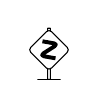
\begin{tikzpicture}[baseline=(x.base)]
		\draw[rounded corners=.01em] (-.05em,-1.07em)rectangle(.05em,.78em);
		\draw[fill=white,rounded corners=1.3] (0,.75em)--(.75em,0)--(0,-.75em)--(-.75em,0)--cycle;
		\draw[line width=0.2mm, line cap=round](-.4em,-1.07em)--(.4em,-1.07em);
		\node(x) at (0,0em) {};
		% Thank you https://tex.stackexchange.com/a/262510
		\draw[
			line cap=but,
			line join=round,
			x=.5em,
			line width=0.5mm,
			y=1*(height("Z")-\pgflinewidth)*(1-sin(10)),
			rotate=-10,
			rounded corners=1.5pt,
		](-0.57, 0.57) -- (0.57, 0.57) -- (-0.57, -0.57) -- (0.57, -0.57);
	\end{tikzpicture}%
}

%%%%%%%%%%%%%%%%%%%%%%%%%%%%%%%%%%%%%%%%%%%% MARGINS
\usepackage{marginnote}
% Thank you https://tex.stackexchange.com/a/472882
% Makes marginnotes always appear on the left, apparently
%
\makeatletter
\long\def\@mn@@@marginnote[#1]#2[#3]{%
	\begingroup
		\ifmmode\mn@strut\let\@tempa\mn@vadjust\else
			\if@inlabel\leavevmode\fi
			\ifhmode\mn@strut\let\@tempa\mn@vadjust\else\let\@tempa\mn@vlap\fi
		\fi
		\@tempa{%
			\vbox to\z@{%
				\vss
				\@mn@margintest
				\if@reversemargin\if@tempswa
						\@tempswafalse
					\else
						\@tempswatrue
				\fi\fi

					\llap{%
						\vbox to\z@{\kern\marginnotevadjust\kern #3
							\vbox to\z@{%
								\hsize\marginparwidth
								\linewidth\hsize
								\kern-\parskip
								%\mn@parboxrestore
								\marginfont\raggedleftmarginnote\strut\hspace{\z@}%
								\ignorespaces#1\endgraf
								\vss
							}%
							\vss
						}%
						\if@mn@verbose
							\PackageInfo{marginnote}{xpos seems to be \@mn@currxpos}%
						\fi
						\begingroup
							\ifx\@mn@currxpos\relax\else\ifx\@mn@currpos\@empty\else
									\kern\@mn@currxpos
							\fi\fi
							\ifx\@mn@currpage\relax
								\let\@mn@currpage\@ne
							\fi
							\if@twoside\ifodd\@mn@currpage\relax
									\kern-\oddsidemargin
								\else
									\kern-\evensidemargin
								\fi
							\else
								\kern-\oddsidemargin
							\fi
							\kern-1in
						\endgroup
						\kern\marginparsep
					}%
			}%
		}%
	\endgroup
}
\makeatother
%
% Mostly for todonotes
\renewcommand{\marginpar}{\marginnote}
%%%%%%%%%%%%%%%%%%%%%%%%%%%%%%%%%%%%%%%%%%%% /MARGINS

\definecolor{nirlightred}{RGB}{250, 220, 220}
\definecolor{nirdarkred}{HTML}{f40000}
\declaretheoremstyle[
	mdframed={
		backgroundcolor=nirlightred,
		linecolor=nirdarkred,
		rightline=false,
		topline=false,
		bottomline=false,
		linewidth=2pt,
		innertopmargin=5pt,
		innerbottommargin=8pt,
		innerleftmargin=8pt,
		leftmargin=-2pt,
		skipbelow=2pt,
		nobreak
	},
	headfont=\normalfont\bfseries\color{nirdarkred}
]{nirredbox}

% \makeatletter
% \declaretheorem[
% 	style=nirredbox,
% 	name=Warning,
% 	sibling=thm,
% 	% without \leavevmode, the first item in a list gets misformatted
% 	postheadhook={\leavevmode\marginnote{\nirwarnsymbol}[-3pt]%
% 	\ifthmt@thisistheone% restatable makes alignment weird
% 		\hspace{-2.2pt}%
% 	\fi}
% ]{warn}
% \makeatother

\newcommand{\nirideasymbol}{%
	
\begin{tikzpicture}[baseline=(x.base)]
		\draw[rounded corners=.01em] (-.05em,-1.07em)rectangle(.05em,.78em);
		\draw[fill=white,rounded corners=1.3] (0,.75em)--(.75em,0)--(0,-.75em)--(-.75em,0)--cycle;
		\draw[line width=0.2mm, line cap=round](-.4em,-1.07em)--(.4em,-1.07em);
		\node(x) at (0,0em) {};
		\node at (0,0em) {{\textbf{!}}};
	\end{tikzpicture}%
}
\renewcommand{\nirwarnsymbol}{%
	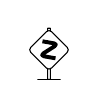
\begin{tikzpicture}[baseline=(x.base)]
		\draw[rounded corners=.01em] (-.05em,-1.07em)rectangle(.05em,.78em);
		\draw[fill=white,rounded corners=1.3] (0,.75em)--(.75em,0)--(0,-.75em)--(-.75em,0)--cycle;
		\draw[line width=0.2mm, line cap=round](-.4em,-1.07em)--(.4em,-1.07em);
		\node(x) at (0,0em) {};
		% Thank you https://tex.stackexchange.com/a/262510
		\draw[
			line cap=but,
			line join=round,
			x=.5em,
			line width=0.5mm,
			y=1*(height("Z")-\pgflinewidth)*(1-sin(10)),
			rotate=-10,
			rounded corners=1.5pt,
		](-0.57, 0.57) -- (0.57, 0.57) -- (-0.57, -0.57) -- (0.57, -0.57);
	\end{tikzpicture}%
}
\makeatletter
\declaretheorem[
	style=nirredbox,
	name=Idea,
	sibling=thm,
	% without \leavevmode, the first item in a list gets misformatted
	postheadhook={\leavevmode\marginnote{\nirideasymbol}[-3pt]%
	\ifthmt@thisistheone% restatable makes alignment weird
		\hspace{-2.2pt}%
	\fi}
]{idea}

\declaretheorem[
	style=nirredbox,
	name=Warning,
	sibling=thm,
	% without \leavevmode, the first item in a list gets misformatted
	postheadhook={\leavevmode\marginnote{\nirwarnsymbol}[-3pt]%
	\ifthmt@thisistheone% restatable makes alignment weird
		\hspace{-2.2pt}%
	\fi}
]{warn}
\makeatother

\title{Calc III Section Notes with Answers
\\ 
\vspace{0.4cm}
\large Spring 2026}




\date{\today}
\author{Hui Sun}


\begin{document}

\maketitle
\tableofcontents

% \tableofcontents
\newpage

\chapter{The Geometry of Euclidean Spaces}


\section*{\centering Week 1 (1/19-23)}



% \begin{center}
%     \Large Calc III-Week 1 )
% \end{center}

\renewcommand\thesection{\arabic{section}}
\noindent
\textbf{Logistics}


\begin{itemize}
    \item TA: Hui.
    \item Email: hsun95@jh.edu.
    \item Office Hours: Tuesday 4-6 PM, Krieger 211; Friday 1-2 PM Zoom.
    \item Biweekly Quizzes: 15 min, 10\%.
    \item Attendance: 5\%. (If you can't make it, email me).
\end{itemize}


\begin{defn}[standard basis of $\R^3$]
    The following vectors 
    \begin{equation*}
        i=(1,0,0), j=(0,1,0), k=(0,0,1)
    \end{equation*}
    are called the \textbf{standard basis} vectors of $\R^3$, and for any vector $a=(a_1,a_2,a_3)\in\R^3$, we can write 
    \begin{equation*}
        a=a_1i+a_2j+a_3k
    \end{equation*}
\end{defn}



\begin{defn}[dot product]
    Let $v=(v_1,v_2,v_3), w=(w_1,w_2, w_3)\in\R^3$, the \textbf{dot product} $v\cdot w$ is given by 
    \begin{equation*}
        v\cdot w=v_1w_1+v_2w_2+v_3w_3
    \end{equation*}
    Alternatively,
    \begin{equation*}
        v\cdot w=\|v\|\|w\|\cos\theta
    \end{equation*}
    where 
    \begin{equation*}
        \theta=\arccos\left(\frac{v\cdot w}{\|v\|\|w\|}\right)
    \end{equation*}
\end{defn}

\begin{defn}[length of vector]
    Let $v=(v_1,v_2,v_3)\in\R^3$, the \textbf{length} or \textbf{norm} of $v$, denoted as $\|v\|$, is 
    \begin{equation*}
        \|v\|=\sqrt{v_1^2+v_2^2+v_3^2}=\sqrt{v\dot v}
    \end{equation*}
\end{defn}

\begin{defn}[linear combination]
    Let $v, w\in\R^3$, a \textbf{linear combination} of $v,w$ is a sum 
    \begin{equation*}
        av+bw
    \end{equation*}
    for some $a,b\in\R$. One can generalize this definition to $n$ vectors: let $v_1, v_2\dots, v_n\in\R^3$, a linear combination of these vectors is a finite sum 
    \begin{equation*}
        a_1v_1+a_2v_2+\dots+a_nv_n
    \end{equation*}
    for some $a_i\in\R, 1\leq i\leq n$. 
\end{defn}


\begin{prop}[properties of the dot product]
    Let $a,b,c\in\R^n$, then 
    \begin{enumerate}
        \item[(a)] Nonnegativity: $a\cdot a\geq 0$, and $a\cdot a=0$ if and only if $a=0$.
        \item[(b)] Scalar multiplication: let $\lambda\in\R$, then 
        \begin{equation*}
            \lambda(a\cdot b)=\lambda a\cdot b=a\cdot \lambda b
        \end{equation*}
        \item[(c)] Distributivity:
        \begin{equation*}
            a\cdot(b+c)=a\cdot b+a\cdot c, \quad (a+b)\cdot c=a\cdot c+b\cdot c
        \end{equation*}
        \item[(d)] Symmetry: $a\cdot b=b\cdot a$.
    \end{enumerate}
\end{prop}


% \noindent
% \textbf{Icebreaking Activity}
% \begin{itemize}
%     \item In a group of three or four: 
%     \begin{enumerate}
%         \item Learn each other names, year, pronouns.
%         \item Find something in common and different among you and share with the entire class.
%         \item Play Buzz if you have time, with prime $7$: say the number if it doens't contain or is not divisible by $7$, say buzz otherwise.
%     \end{enumerate}
% \end{itemize}


\begin{prob}
    Draw the following vectors in $\R^2$:
    \begin{equation*}
        u=(1,2), \quad v=(3,-2)
    \end{equation*}
    Compute $u+v, u-v$, and draw them in the plane.
\end{prob}
\begin{proof}
    \begin{equation*}
        u+v=(4,0), \quad u-v=(-2, 4)
    \end{equation*}
\end{proof}

\begin{prob}
    Consider the following vectors in $\R^3$:
    \begin{equation*}
        u=(1,2,3), \quad, v=(-2, 1, 4)
    \end{equation*}
    \begin{enumerate}
        \item Compute their norms.
        \item  Two vectors $a,b\in\R^3$ are called \textbf{orthognal} if $a\cdot b=0$. Are $u,v$ orthogonal? If not, find a nonzero vector orthogonal to $u$.
    \end{enumerate}
\end{prob}
\begin{proof}
    \begin{enumerate}
        \item \begin{equation*}
            \|u\|=(u\cdot u)^\frac{1}{2}=\sqrt{14}, \quad \|v\|=\sqrt{21}
        \end{equation*}
        \item We check 
        \begin{equation*}
            u\cdot v=-2+2+12=12\neq 0
        \end{equation*}
        thus not orthogonal. A vector that is orthognal to $u$: $(-3,0,1)$. Note that this vector is \textbf{not} unique! For example, $(-1,-1,1)$ is another such vector.
    \end{enumerate}
\end{proof}


\begin{prob}
    Can you express $w=(1,0)$ as a linear combination of $v_1,v_2$ for difference choices of $v_1,v_2$?
    \begin{enumerate}
        \item $v_1=(1,1), v_2=(-2,-2)$.
        \item $v_1=(2,1), v_2=(-1, 0)$.
    \end{enumerate}
\end{prob}






\newpage

\section*{\centering Week 2 (1/26-30)}



\begin{defn}[cross product]
    Let $a,b\in\R^3$, write $a=(a_1,a_2,a_3), b=(b_1,b_2,b_3)$, then the \textbf{cross product}
    \begin{equation*}
        a\times b=\det\begin{bmatrix}
            i&j&k\\
            a_1&a_2&a_3\\
            b_1&b_2&b_3
        \end{bmatrix}
    \end{equation*}
    where $i,j,k$ are the standard vectors in $\R^3$.
\end{defn}


\begin{prop}[properties of the cross product]
    We have the following properties regarding the cross product: let $a,b\in\R^3$,
    \begin{enumerate}
        \item $a\times a=0$.
        \item $a\times b=-b\times a$.
        \item $(a+b)\times c=a\times c+b\times c$, and $a\times (b+c)=a\times b+a\times c$.
        \item $(\alpha a)\times b=\alpha(a\times b)$ for any $a\in\R$.
        \item $a\times b$ is perpendicular to vectors $a,b$.
        \item The length of the cross product is the area of the parallelogram:
        \begin{equation*}
            \|a\times b\|=\|a\|\|b\|\sin\theta
        \end{equation*}
        where $0\leq\theta\leq\pi$ is the angle between them. 
        \item $a\times b=0$ iff $a,b$ are parallel or either $a$ or $b$ are $0$.
        \item The cross product is \textbf{not} associative! For example, compute 
        \begin{equation*}
            (i\times i)\times j, \quad i\times (i\times j)
        \end{equation*}
    \end{enumerate}
\end{prop}



\end{document}